\documentclass[12pt]{article}

% --- Präambeln ---
\input{preamble_2.tex}
%-------------------GENERAL--------------------
\usepackage{amsmath,latexsym, amssymb, dsfont}
\usepackage{braket}

%-------------------UNITS--------------------
\usepackage{siunitx}
\DeclareSIUnit{\Mpc}{Mpc}
\DeclareSIUnit{\solarMass}{\ensuremath{M_\odot}}
\DeclareSIUnit{\erg}{erg}
\DeclareSIUnit{\year}{yr}
\DeclareSIUnit{\nats}{nats}

%------------------SHORTCUTS-------------------

\newcommand{\mean}{\overset{-}{T}}
\newcommand{\degree}{^{\circ}}

\newcommand{\inv}{^{-1}}

\newcommand{\sinc}{\text{sinc}}
\newcommand{\const}{\text{const}}

\newcommand{\Lp}{\text{L}}
\newcommand{\Hilbert}{\mathcal{H}}

\newcommand{\N}{\mathbb{N}}
\newcommand{\Z}{\mathbb{Z}}
\newcommand{\R}{\mathbb{R}}
\newcommand{\C}{\mathbb{C}}

\newcommand{\0}{\hat{\mathbf{0}}}
\newcommand{\1}{\hat{\mathds{1}}}

% Inner and outer product
\newcommand{\ip}[2]{\bra{#1}\!\!\ket{#2}}
\newcommand{\op}[2]{\ket{#1}\!\!\bra{#2}}

\newcommand{\norm}[1]{\lVert #1 \rVert}

%-------------MATRIX ENVIRONMENTS-------------

% Three matrix types [], (), ||, chosen by options b, p, v. Standard ist b.
\newcommand{\bmat}[1]{\begin{bmatrix} #1 \end{bmatrix}}
\newcommand{\pmat}[1]{\begin{pmatrix} #1 \end{pmatrix}}
\newcommand{\vmat}[1]{\begin{vmatrix} #1 \end{vmatrix}}
%-------------THEOREM ENVIRONMENTS-------------

%Hier bei Bedarf Definitionen der Theorem-Umgebungen. 

% ---------- Frontmatter ----------

\title{Title}
\author{Your Name}
\date{\today}

\begin{document}

\maketitle

\selectlanguage{english}
\begin{abstract}
Abstract text.
\end{abstract}

\selectlanguage{german}
\begin{abstract}
Abstract text.
\end{abstract}

% ---------- Mainmatter ----------

\selectlanguage{english}
\section{Nomenclature}

\begin{enumerate}
    \item   SKA: Square Kilometer Array
    \item   EoR: Epoch of Reionization
    \item   SBI: Simulation-Based Inference
    \item   CNN: Convolutional Neural Network
    \item   MLP: Multilayer Perceptron
    \item   KL: Kullback-Leibler divergence
    \item   SM: Standard Model
    \item   WDM: Warm Dark Matter
    \item   $\Lambda$CDM: Lambda Cold Dark Matter
    \item   IGM: Intergalactic Medium
    \item   CLT: Central Limit Theorem
    \item   MI: Mutual Information 
    \item   CE: Conditional Entropy
\end{enumerate}

\section{Introduction}

Give the cosmological setting, small intro to the EoR, and the 21 cm signal. Then introduce the problem of parameter inference, and how it is usually done. Then introduce the idea of using machine learning for this problem, and how it can be done in a more interpretable way. 

The SKA and why simulations are needed. 

SBI in general and why it is needed in this field.

Latent space and geometry.
\section{Physics Background}

A few topics:
    - short introduction to history of universe
    - then focus on EoR
    - 21 cm signal from QM and how it can be used to learn about the EoR

\red{Still need some more subsections to explain the other parameters being examined}

\subsection{The Cosmological Setting}

For the purposes of this thesis, a flat $\Lambda$CDM cosmology with an additional warm dark matter parameter is assumed. The $\Lambda$CDM-model is based on the Friedmann-Robertson-Walker metric:
\begin{align}
    ds^2 = -dt^2 + a^2(t) \biggl(\frac{dr^2}{1-k r^2} + r^2 \bigl(d\theta^2 + \sin^2\theta d\phi^2\bigr)\biggr).
\end{align}
where $a(t)$ is the dimensionless scale factor and $k$ is the curvature constant.

Combined with Einstein's field equations and the assumption that the universe may be described as a perfect fluid, the dynamics of this universe are described by the Friedmann equations:
\begin{align}
\left( \frac{\dot{a}}{a} \right)^2 &= \frac{8 \pi G}{3} \rho + \frac{\Lambda}{3} - \frac{k}{a^2},\\
 \quad \frac{\ddot{a}}{a} &= -\frac{4 \pi G}{3} (\rho + 3p) + \frac{\Lambda}{3}.
\end{align}
where $G$ is Newton's constant, $\Lambda$ is the cosmological constant and $\rho$ is the energy density of the universe. The scale factor as well as the energy density are time-dependent quantities.

The ratio $H = \dot{a}/a$ is called the Hubble parameter and measures how fast the universe is expanding in the following sense: given two observers at $(t_1, r_1), (t_2, r_2)$ in a FRW-universe, where observer 1 emits a signal of duration $\Delta t_1$, observer 2 seeds a scale-factor dependent dilation of the signal duration, as measured by the cosmological redshift:
\begin{align}
    z = \frac{\Delta t_2}{\Delta t_2} - 1 = \frac{a(t_2) - a(t_1)}{a(t_1)} > 0 \quad \text{if universe expanding}
\end{align} 
In the limit of $t_2 \rightarrow t_1$, if $d$ is the instantaneous distance between the observers, one then has
\begin{align}
    z \approx \frac{\dot{a}}{a} \biggl|_{t_1} d + \mathcal{O}((t_1-t_2)^2)
\end{align}
such that $H$ measures the expansion rate at a given time in units $\si{1/s}$.

\red{Now a part on matter densities}

The six parameters describing the $\Lambda$CDM-model and their estimated values today are shown in table~\ref{tab:LCDM_params}.

\red{See PieNET paper:}

All other cosmological parameters are fixed to the Planck measurements, assuming flat-
ness and a cosmological constant. This means Ωb = 0.04897, $\sigma_8$ = 0.8102, h= 0.6766, and
ns
= 0.9665.

\red{These are not the fundamental params. Choose which exactly to include.}
% \begin{table}[caption={Parameters of  $\Lambda$CDM with estimated values}, label={tab:LCDM_params}]
%     Name & Symbole & Value & Unit & Source \\
%     Hubble constant & $H_0$ & 67.4 & \si{\kilo\meter\per\second\per\Mpc} & Planck 2018 \\
%     Matter density & $\Omega_m$ & $0.315 \pm 0.007$ & & Planck 2018 \\
%     Dark energy density & $\Omega_\Lambda$ & 0.685 & & Planck 2018 \\
%     Spectral index & $n_s$ & 0.965 & & Planck 2018 \\
%     Matter fluctuation amplitude & $\sigma_8$ & $0.811\pm0.006$ & & Planck 2018 \\
%     Equation of state & $w$ & -1 & & Planck 2018 \\
% \end{table}

\begin{table}[htbp]
\centering
\caption{Parameters of  $\Lambda$CDM with estimated values}
\label{tab:LCDM_params}
\begin{tabular}{l c c c c}
\toprule

Name & Symbole & Value & Unit & Source \\
\midrule
Hubble constant & $H_0$ & 67.4 & \si{\kilo\meter\per\second\per\Mpc} & Planck 2018 \\
Matter density & $\Omega_m$ & $0.315 \pm 0.007$ & & Planck 2018 \\
Dark energy density & $\Omega_\Lambda$ & 0.685 & & Planck 2018 \\
Spectral index & $n_s$ & 0.965 & & Planck 2018 \\
Matter fluctuation amplitude & $\sigma_8$ & $0.811\pm0.006$ & & Planck 2018 \\
Equation of state & $w$ & -1 & & Planck 2018 \\

\bottomrule
\end{tabular}
\end{table}

\red{Cite a few papers that give the current status of cosmology in $\Lambda$CDM, e.g. Planck 2018, etc.}

\red{Cite current values for all params that will be inferred}

According to the cosmological standard model, the timeline of the universe is approximately as follows:

The first phase of the universe is marked by \textit{radiation domination}. Immediately after the Big Bang, the universe underwent a period of rapid expansion called \textit{inflation}, during which space expanded by appriximately an order of $10^{26}$. This inflation was driven by the so-called inflaton field. During the following process of reheating, the energy of the inflaton field was converted to SM particles, which enabled subsequent \textit{baryogenesis}, i.e. the creation of matter and antimatter particles. In the subsequent annihilation of matter.antimatter pairs, a small excess of matter paticles survived, composing the matter content of the universe today. There have been many proposed mechaninisms for both reheating and baryogensesis, and both are active fields of research. \red{Insert sources here} In the following time scale of $20\cdot 10^{-12}\si{\s} - 1000\si{\s}$, particles acquired mass and coalesced into hadrons. Neurinos decoupled from baryons and thus the cosmic neutrino background was formed. What followed was an epoch named \textit{big bang nuceosynthesis}, during which mostly protons and neutrons bound to primordial nuclei, consisting mostly of hydrogen, Helium-4 and traces of deuteron, Helium-3 and lithium. 

The second phase of the universe is marked by \textit{matter domination}. During \textit{recombination}, electrons and nuclei where bound to neutral atoms. Photons were no longer in thermal equilibrium with matter and thus ”decouple”, forming the cosmic microwave background (CMB). Measurements of the CMB today provide one of the most crucial constraints on cosmological parameters.

After recombinations, most photons propagate freely and are quickly redshifted, such that the universe becomes dark. This period is therefore called the \textit{dark ages}. Matter has not yet coalesced into stars and galaxies. The main source of photons \red{visible phtons?} is the 21 cm emission line of neutral hydrogen. 

Once first stars and galaxies have formed, they emit photons energetic enough to ionize the surrounding hydrogen. This period is called the \textit{epoch of reionization} (EoR). By the end of the EoR, most of the IGM is ionized and continues to be so today.

\red{Need small intro on warm dark matter}


\red{These sections are based on}
% \cite{PDG_2024}

\red{Maybe short example of how an evolution might be described...}


\red{How other cosmological models can be tested with the EorFlow setup, maybe also put this somewhere else.}

\red{What is matter distribution at the redshift when beginning study?}

\red{Brief summary of CMB}

\red{Small overview of existing studies of timeline of universe, why there is a gap in EoR}

\red{Maybe cite more recent paper that explains why studying this exact regime of redshifts}

\subsection{The Astrophysical Setting}


\subsection{On the Origin of the 21 cm Signal}

Temperature of the ISM at around these redshifts, why neutral hydrogen does not absorb of emit visible light at these temperatures.

How trace elements interact with visible light at these temperatures.

At least mention the possibility of a derivation 

Quantum mechanical aspect: hyperfine splitting of ground state of hydrogen.

Statistical mehanics aspect: spin temperature and how it is useful in measuring the 21 cm signal.

    - Einstein coefficients from QM
    - Different processes that influence the spin temperature, e.g. collisional coupling, Wouthuysen-Field effect, etc.
    - Final formula for spin temperature

\subsection{Evolution of the 21 cm Signal}


\section{Physics of the 21cm Signal}
For the purposes of this thesis, a flat $\Lambda$CDM cosmology with an additional warm dark matter parameter is assumed. The cosmological setting is that of the matter-dominated universe after recombination, during which the CMB was formed. During this time, most photons propagate freely and are quickly redshifted, such that the universe becomes dark. This period is therefore called the Dark Ages. Matter has not yet coalesced into stars and galaxies. Once first stars and galaxies have formed, they emit photons energetic enough to ionize the surrounding hydrogen. This period is called the Epoch of Reionization. By the end of the EoR, most of the IGM is ionized and continues to be so today.

This section covers $21~\si{cm}$ line of neutral hydrogen and how the $21~{cm}$ from this cosmological period has evolved until today. It is based on~\cite{fundamentals}.

\subsection{The origin of the 21cm signal}
The two electron spin states of neutral hydrogen in the $1s$ state have slightly different energy levels. This hyperfine structure originates from the parallel (triplet state) and antiparallel (singlet state) orientation of electron spin with respect to the nucleus. The transition between states is forbidden, the excited state having a mean lifetime of $\sim 11\cdot 10^6~\si{yrs}$. The triplet state carries slightly more energy, the energy difference being $\Delta E \approx 10^{-6}~\si{eV}$, which corresponds to a frequency of $\nu \approx 1.42~\si{GHz}$, or a wavelength of $\lambda \approx 21~\si{cm}$. 

Neutral hydrogen gas made up most of baryonic matter during CD and EoR, and $21~\si{cm}$ photons emitted during these epochs can be measured today. A $21~\si{cm}$ photon emitted at some point during CD or EoR is redshifted by the time it reaches the earth. At redshift ranges $z \sim 6-30$ , it is now measured on a range of $\nu\sim 46-200~\si{MHz}$, or $\lambda\sim 1.5-6.5~\si{m}$. This wavelength range belongs to the regime of radio astronomy and is covered by the SKA-Low setup, which is sensitive to frequencies $\nu \sim (50-350)~\si{MHz}$\footnote{See the \href{https://www.skao.int/en/science-users/118/ska-telescope-specifications}{SKAO website}.}.

\subsection{The evolution of the 21cm signal until today}
There are various mechanisms that lead to changes in this spin state of neutral hydrogen in the IGM. Those mechanisms that are consequences of the quantum mechanical properties of the atom are measured by Einstein coefficients, which are introduced in the following. The singlet state is denoted with index $0$ and the triplet state with index $1$. Then the index $01$ denotes excitation, and $10$ de-excitation. 

$A_{10}$ describes spontaneous emission and can be given as a rate. For neutral hydrogen, one finds $A_{10}\approx 2.85\cdot 10^{-15}~\si{s}^{-1}$.

$B_{01/10}$ describes absorption/stimulated emission. For neutral hydrogen, one finds $B_{10} = A_{10}(c^2 /2h\nu^3)$ and $B_{10}g_1 = B_{01}g_0$, where $\nu$ is the $21~\si{cm}$ line frequency given above and $g_i$ is the spin degeneracy factor of each state. In terms of the $21~\si{cm}$ it is used to describe the interaction of neutral hydrogen clouds with CMB radiation.

Two other effects also lead to the (de-)excitation of neutral hydrogen in the IGM, and their rates are described by effective Einstein coefficients. C denotes those processes driven by collision interactions with other hydrogen atoms, free electrons and protons, and P those from scattering with Lyman-$\alpha$ photons. In equilibrium, both define a kinetic temperature $T_K$ and effective color temperature $T_c$:
\begin{align}
    \frac{C_{01}}{C_{10}} &= \frac{g_1}{g_0} e^{-\frac{T_*}{T_K}}\\
    \frac{P_{01}}{P_{10}} &= \frac{g_1}{g_0} e^{-\frac{T_*}{T_c}},
\end{align}
where again $T_K,T_c \gg T_*$ and the exponential can be expressed in first-order Taylor expansion.

On a large scale, the relative populations $n_0$ and $n_1$ of neutral hydrogen atoms in different spin states are described by (or determine) the spin temperature $T_S$:
\begin{align}
    \frac{n_1}{n_0} 
    = \frac{g_1}{g_0} \exp \biggl(-\frac{E_{10}}{k_B T_S}\biggr) 
    \equiv \frac{g_1}{g_0} \exp \biggl(-\frac{T_\star}{T_S}\biggr),~\label{eq:Boltzmann}
\end{align} 
As a reminder, the $g_i$ are spin degeneracy factors and $E_{10}$ the energy difference between spin states. An estimate of $T_S$ allows an estimate of the relative populations. For realistic astrophysical environments, $T_S \gg T_*$ and as such $n_1 \approx 3n_0$ is a working approximation. 

An estimate of $T_S$ is then obtained by a rate balancing of the aforementioned Einstein coefficients:
\begin{align}
    n_1 (A_{10} + B_{10}I_\gamma +C_{10}+P_{10})=n_0(B_{01}I_\gamma + C_{01}+P_{01}),~\label{eq:rate_balancing}
\end{align}
where $I_\gamma$ is the specific intensity of CMB photons at the frequency of the $21~\si{cm}$ line. The CMB background is the source closest resembling a blackbody spectrum, which is in this frequency range described by the Rayleigh-Jeans law, with which $I_\gamma$ can be written in terms of a temperature at the frequency of the $21~\si{cm}$ line. Plugging everything into~\ref{eq:rate_balancing} yields the following approximation to $T_S$:
\begin{align}
    T_S^{-1} &= \frac{T_\gamma^{-1} + x_c T_K^{-1} + x_\alpha T_C^{-1}}{1+x_c+x_\alpha}\\
    x_c &= \frac{C_{10}}{A_{10}}\frac{h\nu}{k_B T_\gamma}\\
    x_\alpha &= \frac{P_{10}}{A_{10}}\frac{h\nu}{k_B T_\gamma}.
\end{align}
This raises the question of what the measured $21~\si{cm}$ looks like, given this estimate of $T_S$. 

The $21~\si{cm}$ signal is given in terms of brightness offset temperature $\delta T_B$ between the CMB and the spin temperatures and is calculated from the specific intensity measured by the radio telescope, assuming the Rayleigh-Jeans regime. This is done with the radiative transfer equation
\begin{align}
    \frac{dI_\nu}{ds} = -\alpha(\nu) I_\gamma + \alpha(\nu) I_S,~\label{eq:specific_intensity}
\end{align}
where $\nu$ is the frequency, $I_\gamma$ denotes the CMB specific intensity, $I_S$ that of the $21~\si{cm}$ signal from the neutral hydrogen cloud and $\alpha(\nu)$ the absorption coefficient of neutral hydrogen.

The observed specific intensity $I_B$ is obtained by solving the radiative transfer equation from~\ref{eq:specific_intensity}, yielding:
\begin{align}
    I_B &= I_S (1-e^{-\tau})+I_\gamma e^{-\tau}\\
    \tau(\nu) &= \int \alpha(\nu) ds,
\end{align}
where $\tau$ is the so-called optical depth. This carries the interpretation that for an optically thick material, $\tau \gg 1$, the signal is dominated by the $21~\si{cm}$ signal and for an optically thin material,  $\tau \ll 1$, by CMB radiation. 

Once again using the Rayleigh-Jeans law to convert this to temperature and adding the redshift correction for the CMB temperature, this yields
\begin{align}
    T_{B0}(1+z) = T_S (1-e^{-\tau})+T_0 (1+z)e^{-\tau}. 
\end{align}
Finally, the brightness offset temperature is obtained by subtracting the CMB background:
\begin{align}
    \delta T_B = T_{B0} - T_0 = \frac{T_S - T_\gamma}{1+z}(1-e^{-\tau}).~\label{eq:delta_T_simple}
\end{align}
The quantity $\tau$ remains to be estimated. The absorption coefficient measures the probability of an interaction per frequency and unit distance. Given an Einstein coefficient X, it is given by 
\begin{align}
    \alpha(\nu) = \frac{h\nu}{c} X n \phi(\nu),
\end{align}
where $n$ is number density of atoms partaking in the interaction and $\phi$ is the line profile normalized to one. Then one finds for neutral hydrogen:
\begin{align}
    \alpha(\nu) 
    &= \frac{h\nu}{c}(B_{01}n_0 - B_{10}n_1)\phi(\nu)\\
    &\approx \frac{h\nu}{c}n_0 B_{01}\frac{h \nu}{k_B T_S}\phi(\nu),
\end{align}
the approximation coming from eq.~\ref{eq:Boltzmann}. The line profile is approximated by $\phi(\nu) \approx c/(s H(z) \nu)$ with $s$ a distance and $H$ the Hubble parameter at redshift z, an estimate made when considering the effect of cosmological recession. Then:
\begin{align}
    \tau(\nu) &= A(\nu) \frac{x_\text{HI}n_H }{T_S H(z)}\\
    A(\nu) &= \frac{3c^2 h A_{10}}{32 \pi \nu^2 k_B},
\end{align}
with $n_H$ the density of hydrogen atoms, for which one can use:
\begin{align}
    n_H = (1+\delta_b) \frac{3H_0^2}{8 \pi G m_p} \Omega_{b,0} (1-Y_\text{He})(1+z)^3,
\end{align}
with $\Omega_{b,0}$ the present-day baryon density, $m_p$ the proton mass, $G$ the gravitational constant, $\delta_b$ the fluctuation of baryon content and $Y_\text{He}$ the fraction in mass in helium.

Assuming matter domination yields $H(z) = H_0 \Omega^{1/2}_{m,0} (1 + z)^{3/2}$ with $H_0$ and $\Omega_{m,0}$ the present-day cosmological constant and matter density parameter, one obtains a more detailed approximation of the brightness offset temperature from~\ref{eq:delta_T_simple} in the limit $\tau \ll 1$:
\begin{align}
    \delta T_B \approx 27~x_{\text{HI}}(1+\delta_b)\biggl(1-\frac{T_\gamma}{T_S}\biggr)
    \biggl(\frac{1+z}{10}\frac{0.15}{\Omega_{m,0}h^2}\biggr)^{1/2}\biggl(\frac{\Omega_{b,0}h^2}{0.023}\biggr)~\si{mK},~\label{eq:brightness_offset_final}
\end{align} 
with $x_{\text{HI}}$ the neutral hydrogen fraction. From the expression in eq.~\ref{eq:brightness_offset_final}, it becomes clear that if $T_S > T_\gamma$, the measured brightness offset is positive and vice versa. 

\subsection{Qualitative behaviour of the 21cm signal}
During the Dark Ages, the expansion of the universe causes the neutral hydrogen gas to cool adiabatically, which causes the absorption signal for $z>30$. As collisions cease in the decreasingly dense gas, absorption stops and $\delta T_B \approx 0$. The emission of first Lyman-$\alpha$ photons causes $T_S < T_\gamma$, resulting in the strong absorption feature but soon thereafter saturating. These first sources also emit X-rays which heat the IGM, resulting in an emission feature. This signal decreases when X-rays have nearly completely heated the IGM, such that the signal is $\delta T_B \approx 0$ by $z\approx 6$ and remains so until today.
\begin{figure}[H]
    \centering
    \includegraphics[width=0.7\linewidth]{graphics/lightcone.png}
    \caption{A map of the $21~\si{cm}$ signal of neutral hydrogen~\cite{fundamentals}}
    \label{fig:lightcone}
\end{figure}


\section{Machine Learning Background}

\red{As an introduction to the methods used in this field, this section covers the concept of neural posterior approximation, some theory behind the class of models analyzed in this thesis as well as a summary of metric from information theory, and how they can evaluate a model's quality.}

In the following, $x$ denotes a data sample, and $\theta$ a corresponding parameter. Probability densities are denoted $p$, and their approximations with $q$. Functions $s$ denote objects that summarize data, so $s(x)$ is such a summary. Neural networks are denoted with an index $\phi or \psi$, so $q_\phi$ is an estimate of a probability distribution done with a neural network, and $s_\psi$ is a summary done by a neural network.

\subsection{Neural posterior estimation}
In a Bayesian inference task, processing these data would typically be done by choosing:
\begin{enumerate}
    \item   a likelihood $p(x|\theta)$ describing how observed data arised from a specific set of parameters,
    \item   a prior $p(\theta)$ describing beliefs about the parameter distribution before seeing data.
\end{enumerate}
Given data d, one then calculates the posterior distribution using Bayes' theorem:
\begin{align}
    p(\theta|x) \sim p(x|\theta) p(\theta).
\end{align}
In many applied cases, an analytic shape of the likelihood is not available. An example is when the data come from a complex simulator. Then one can sample from this simulator and as such from the likelihood, but the expression $p(x_{\text{observed}}|\theta)$ is not obtainable and as such, the posterior cannot be calculated. In such setting, an alternative is to model the posterior separately, such that given $x_{\text{observed}}$, one can at least sample from the posterior: $\theta \sim q(\theta | x_{\text{observed}})$. This is known as likelihood-free inference. When the posterior is approximated using a neural network $q_\phi(\theta |x)$, one also speaks of neural posterior estimation (NPE).

An advantage is that unlike with the traditional Bayesian methods, the posterior does not have to be re-calculated given new data: the neural network simply has to be evaluated on the new dataset. In this way, the cost of obtaining the posterior was payed beforehand during training. This concept is known as amortized inference. In order to train the model, data is needed, and this is where simulators are implemented. The posterior model is trained on simulated data and once trained, one can sample parameters by $\theta \sim q_\phi(\theta | x_{\text{observed}})$. In this way, NPE becomes a way of implementing simulation-based inference.

\subsection{Information Theory and Neural Estimators}
Traditionally, data as complex as those expected from SKA are analyzed using physics-inspired summary statistics $s_\text{phys}(x)$, which map the data to a lower-dimensional space with known interpretation. An example is the power spectrum. Such a summary comes with the benefit of interpretability, but the caveat is a potentially large information loss. This motivates the use of a neural networks to learn a different summary $s_\phi(x)$, and the procedure is then called representation learning. The summarry is hopefully more informative of the parameter of interest, though potentially less interpretable. If $\mathbb{I}$ is a measure of informativeness between the data and the parameters, this increased informativeness can be expressed as:
\begin{align}
    \mathbb{I}(\theta;x) 
    \geq \mathbb{I}(\theta;s_\phi(x)) 
    > \mathbb{I}(\theta;s_{\text{phys}}(x)).
\end{align}
The necessitates a measure of informativeness for use in representation learning, which is introduced in this section.

\subsubsection*{Some Basic Measures in Information Theory}
Given a random variable $X$ distributed as $p$, $X \sim p$, the entropy of $X$ is defined as:
\begin{align}
\mathbb{H}(X) = -\mathbb{E}_{X} \left[ \log p(X) \right] \geq 0.
\end{align}
If the logarithm is chosen with base 2, one defines the unit of this quantity as bits. If one uses the natural logarithm, the entropy is measured in units of nats. 

Entropy is a measure of the uncertainty of a random variable. A high entropy corresponds to a lack of predictability of the random variable's outcome. As an example, the entropy of the uniform distribution is maximal, while that of the delta distribution is zero. One therefore considers entropy to be a measure of the amount of information contained in the random variable's distribution.

The generalization to conditional entropy is:
\begin{align}
    \mathbb{H}(X|Y) =  -\mathbb{E}_{X, Y} \left[ \log p(X|Y) \right]
\end{align} 

Another important metric in information theory is the Kullback-Leibler divergence. Let $X \sim p$ and $Y \sim q$ be two random variables over the same sample space. The KL-divergence between $p$ and $q$ is defined as:
\begin{align}
\mathbb{D}_{\text{KL}}(p || q) = \mathbb{E}_{X} \left[ \log p(X) - \log q(X) \right] \geq 0
\end{align}
The KL-divergence satisfies the identity axiom, $\mathbb{D}_{\text{KL}}(p || q) = 0 \Leftrightarrow p = q$. It is not symmetric and does not satisfy the triangle inequality and as such is not a metric. However, it does still carry an interpretation as a distance between two probability distributions: from the above expression it is clear that the more $q$ resembles $p$, the smaller the measured KL-divergence becomes. A smaller the KL-divergence between the two distributions means there is less information loss by using  $q$ to approximate $p$.

Since the KL-divergence is assymmetric, one distinguishes $\mathbb{D}_{\text{KL}}(p || q)$ as the forwards KL between $p$ and $q$, and $\mathbb{D}_{\text{KL}}(q || p)$ as the backwards KL between $p$ and $q$. Minimizing the forwards KL-divergence between the data distribution and the model distribution is equivalent to maximizing the negative log-likelihood, because
\begin{align}
    \mathbb{D}_{\text{KL}}(p_{\text{data}} || q_\phi) = 
    -\mathbb{H}(p_{\text{data}}) - \E_{x \sim p_{\text{data}}} 
    \bigl[ \log q_\phi \bigr] = \text{NLL} + \text{const}
\end{align}

Lastly, the mutual information between two random variables $X$ and $Y$ is defined as:
\begin{align}
\mathbb{I}(X; Y)
         &= \mathbb{D}_{\text{KL}}(p(X, Y) || p_X(X) p_Y(Y)) \geq 0.
\end{align}
An alternative formulation in terms of entropy is:
\begin{align}
    \mathbb{I}(X; Y) = \mathbb{H}(X) - \mathbb{H}(X | Y) 
    = \mathbb{H}(Y) - \mathbb{H}(Y | X).
\end{align}
Mutual information is symmetric and nonnegative. It is zero if and only if $X$ and $Y$ are independent and becomes maximal if and only if $X = Y$. One interprets its value as the amount of information obtained about one random variable while observing another. Since it is defined as an expectation over the joint distribution of the two variables $X$ and $Y$, it is sensitive to higher moments of these distributions, and cannot be captured simply be e.g. their variance.

\subsubsection*{Mutual Information Estimation}
In the context of representation learning, mutual information can be used as a measure of model quality. This is motivated by the data processing inequality, which in this context can be phrased as follows:

Let $X$, $Y$ and $Z$ denote random variables. These are processed as $X \rightarrow Y \rightarrow Z$, in the sense that a sample from $X$ is processed to produce a sample from $Y$, which in turn is processed to produce a sample from $Z$, without any additional knowledge of $X$. Then $Z$ cannot contain more information about $X$ than $Y$, so
\begin{align}
    \mathbb{I}(X;Y) \geq \mathbb{I}(X;Z).
\end{align}
This applied in the context of SBI and NPE, where the parameters of interest $\theta$ are part of the first random variable, the simulated data $x$ part of the second and the summarized data $s_\phi(x)$ part of the third. The data processing inequality then reads:
\begin{align}
    \mathbb{I}(\theta;x) 
    \geq \mathbb{I}(\theta;s_\phi(x)),
\end{align}
and this explains why mutual information is the needed measure of informativeness mentioned in the beginning of this section. A good summary keeps as much information about the original data as possible, subject to the constraint that it should contain less total information than the data itself, i.e. summarize it in some way. The summary distribution is also referred to as the bottleneck.

\red{Something on information bottleneck method?}

In practice, mutual information between the bottleneck $Z$ and the parameter distribution $\Theta$ can only be estimated. In the setting of NPE, one can use the learned posterior to estimate mutual information in a natural way, described in the following. The mutual information between the bottleneck and the parameter distributions is defined as
\begin{align}
    \mathbb{I}(\Theta; Z) &= \int p(\theta, z) \log \frac{p(\theta|z)}{p(\theta)}~\label{eq:MI_int},
\end{align}
where the distribution $p(\theta|z)$ is now estimated by a learned $q_\phi(\theta|z)$, the optimization objective being to minimize the KL-divergence $\mathbb{D}_{\text{KL}}(p||q_\phi)$. The Monte-Carlo approximation of eq.~\ref{eq:MI_int} using this distribution is referred to as the Barber-Agakov estimate~\cite{Barber_2003}:
\begin{align}
    \hat{\mathbb{I}}(\Theta;Z) = \mathbb{I}_{\text{BA}}(\Theta;Z) = \E_{P(\Theta,Z)} \left[ \log q_\phi(\theta|z) - \log p(\theta) \right].
\end{align}
This is computable, because the distribution of the prior $p(z)$ can in practice either be ignored as a constant factor, or in case of SBI is chosen and therefore known. If this is not the case, $p(z)$ can also be estimated separately, which however introduces more uncertainty in the above estimate.

Because the KL-divergence is non-zero, the BA-estimate yields a lower bound on the true mutual information:
\begin{align}
    \mathbb{I}(\Theta;Z) \geq \mathbb{I}_{\text{BA}}(\Theta;Z)
\end{align}

\subsection{An architecture for complex data}

The model discussed in the previous section can be implemented with various different architectural choices. One important choice is that of the \textit{bottleneck size}, that is, the dimensionality of the CNN's output. This part of the model is referred to as the bottleneck because it is the point in which the data are compressed to the highest degree. While a larger bottleneck should be able to capture more information about the data, one needs a principled way to balance the increased model complexity with the increase in information captured by the model. One way to do this is to evaluate the \textit{mutual information} between the feature and the bottleneck space across different such bottleneck dimensions. Mutual information and it's estimation are introduced in the following sections.


An architecture that has proven to be successful in recent SBI approaches \red{some citations here} combines two neural networks in the following principle:
\begin{enumerate}
    \item   The image data are used as input for a convolutional neural network (CNN), which compresses these into a much lower-dimensional summary.
    \item   This summary is mapped to whichever feature is being inferred by a conditional normalizing flow (CNF).
\end{enumerate}
The idea is that the CNN learns to efficiently encode any relevant physics information, while the flow learns to interpret the CNN's output and map it to the inferred quantity. These two networks are introduced in the following.

\subsubsection*{Convolutional Neural Networks}

CNNs are inspired by the task of implementing neural networks in image analysis, i.e. on data with 2D spatial structure. An early version was successfully implemented in 1983 with Fukushima's ”Neucognitron”~\red{Neocognitron citation}. An architecture implementing backpropagation was LeCun's ”LeNet”~\red{LeNet citation}.

To explain the novel concepts behind the CNN in comparison with a MLP, the CNN architecture will first be discussed in 1D. The generalization to higher dimensions will be discussed afterwards.

Let $X$ denote the \red{data space} and $Y$ the feature space. 

Let the input have dimensions $x \in \R^{C\times H \times W}$ where C the channel dimension, H the height dimension and W the width dimension. In case of an RGB image, this channel dimension would be three. 

The CNN learns a function $f_\theta: X \rightarrow Y$. 

As opposed to a simple MLP, the CNN offers the following advantages:

\red{Using summation convention}

\red{Not writing bias explicitly}

A basic MLP consists of only one type of layer. If $h$ is the output of the previous layer, the current layer is defined by
\begin{align}
    z_i = \phi(W_{ij} h_j),
\end{align}
The CNN implements additional layers.

A convolutional layer applies a convolution operaton:

\red{Talk abt convolution vs cross-correlation here}

\red{Is this def even correct? Not need different indices on h?}
\begin{align}
    z_i = \phi(\left[w \circledast h\right]_i) = \phi(\sum_k w_k h_{i+k})
\end{align}
where the dimensionality of the kernel $w\in \R^K$ is typically much lower than that of the data.

A pooling layer applies a pooling operation:
\begin{align}
    z_i = \operatorname{pool} K_{ij}h_j
\end{align}
where $K$ defines a pooling window for each index $i$. Typical choices for $\operatorname{pool}$ are $\operatorname{maxpool}$, which chooses the maximum of all given values, or $\operatorname{meanpool}$, which calculates their mean.

\red{The purpose of a pooling layer is to...}

\red{Add normalization layers here}

\red{Add info on stride params etc here}

\red{Hier kann man schon ein bisschen mehr schreiben, this is all very basic. More info on the CNN specific to this project to come.}

\red{Put it together here, potentially add image of total architecture.}

\red{Also missing MSE loss function as usual loss}

\subsubsection*{Conditional Normalizing Flows}

A normalizing flow is a model that learns to transform a simple (often Gaussian) distribution into a more complex one, the target distribution. The transformation is chosen to be invertible, such that the model becomes generative: once trained, it can be inverted and by transforming samples from the normal, one can sample from the approximated target distribution.

Let $u \sim p_u = \mathcal{N}(0, I_n)$ with $n \in \N$ the base distribution and $x \sim p_x$ with $p_x$ the $n$-dim. target distribution. Let $f: \R^n \to \R^n$ a diffeomorphism, with $g = f^{-1}$ its inverse. The training objective is to find $g$, such that
\begin{align}
    u = g(x) \sim p_u, \qquad x \text{ sampled from } p_x.
\end{align}
The process of generating samples from the approximated distribution is the inverse of the above:
\begin{align}
x = f(u) \sim q_x, \qquad u \text{ sampled from } p_u.
\end{align}
For a given transformation, one computes $p_x(x)$ by applying the change of variables formula:
\begin{align}
q_x(x) = p_u(g(x)) \left| \det \left( \frac{\partial g(x)}{\partial x} \right) \right| = p_u(u) \left| \det \left( \frac{\partial f(u)}{\partial u} \right) \right|^{-1}.
\end{align}
The NLL is the loss function used for optimization, which then becomes:
\begin{align}
    \mathcal{L}_{\text{NF}} = - \E_{x \sim p_x} \Biggl[ \frac{|g(x)|^2}{2} + 
    \log \left| \det \left( \frac{\partial g(x)}{\partial x} \right) \right|\Biggr]
\end{align}
where the first term is a regularization for the latent (in this case Gaussian) space and the second stems from the transformation. See \red{cite Plehns book} for more details.

The normalizing flow becomes expressive by allowing the transformation to be as complex as possible, while restricting it to a class of functions with efficiently computable Jacobian determinants makes it computationally tractable. In practice, one often models $g$ as a composition of simple neural networks, e.g. multilayer perceptrons. \red{How these are invertible...}

\red{Next few lines could also just be skipped}

Let $g_\theta = g_1 \circ g_2 \circ ... \circ g_k$ with $g_i: \R^n \to \R^n, x \mapsto g_i(x | \theta_i)$ and $k \in \N$. 

Now the loss becomes
\begin{align}
    \text{NLL}_\theta =  \sum_{i=1}^{k} \log \left| \det J(g_i) \right| - \log p_u (g_\theta(x))
\end{align}

\red{How to ensure it is a probabilistic model?}

\red{Come up with nicer notation for $g_i (\cdot | \theta_i)$}

\red{Now what this specific Freia flow does. Research on website!}


\section{Basic Neural Networks}

EoRFlow general description, goal etc. Why it is needed. Have figure of architecture.

How this type of model can be used in 21 cm cosmology in general, and then how it is used here specifically.

Traditionally, data as complex as those expected from SKA are analyzed using summary statistics. A summary statistic is a function that maps the data to a lower-dimensional space, typically with some physical interpretation. An example is the power spectrum. The interpretation of the power spectrum is \red{blablabla}. However the power spectrum \red{is not a sufficient statistic} for the 21 cm signal. As an alternative, one can use a neural network to learn a summary statistic of the data. While being potentially more informative, this comes at the cost of less interpretability.

For cnn and flow:
    - general stuff on model
    - architecture, where it's inspired from, how it was adapted to the problem, etc
    - loss function
    - backpropagation 

Training
    - details on scheduler, optimizer, etc
    - training hyperparameters, chip used

Why is a generative model needed? Why is the flow chosen? What are the advantages of flows over other generative models?

Why this very specific architecture?

\red{Do I want a short ML intro? Could e.g. introduce MLP here and rename section to NNs in general}

\red{A word about how architectures will be discussed, e.g. notation with h, z, x, etc.}

\subsection{Convolutional Neural Networks}

CNNs are inspired by the task of implementing neural networks in image analysis, i.e. on data with 2D spatial structure. An early version was successfully implemented in 1983 with Fukushima's ”Neucognitron”~\red{Neocognitron citation}. An architecture implementing backpropagation was LeCun's ”LeNet”~\red{LeNet citation}.

To explain the novel concepts behind the CNN in comparison with a MLP, the CNN architecture will first be discussed in 1D. The generalization to higher dimensions will be discussed afterwards.

Let $X$ denote the \red{data space} and $Y$ the feature space. 

Let the input have dimensions $x \in \R^{C\times H \times W}$ where C the channel dimension, H the height dimension and W the width dimension. In case of an RGB image, this channel dimension would be three. 

The CNN learns a function $f_\theta: X \rightarrow Y$. 

As opposed to a simple MLP, the CNN offers the following advantages:

\red{Using summation convention}

\red{Not writing bias explicitly}

A basic MLP consists of only one type of layer. If $h$ is the output of the previous layer, the current layer is defined by
\begin{align}
    z_i = \phi(W_{ij} h_j),
\end{align}
The CNN implements additional layers.

A convolutional layer applies a convolution operaton:

\red{Talk abt convolution vs cross-correlation here}

\red{Is this def even correct? Not need different indices on h?}
\begin{align}
    z_i = \phi(\left[w \circledast h\right]_i) = \phi(\sum_k w_k h_{i+k})
\end{align}
where the dimensionality of the kernel $w\in \R^K$ is typically much lower than that of the data.

A pooling layer applies a pooling operation:
\begin{align}
    z_i = \operatorname{pool} K_{ij}h_j
\end{align}
where $K$ defines a pooling window for each index $i$. Typical choices for $\operatorname{pool}$ are $\operatorname{maxpool}$, which chooses the maximum of all given values, or $\operatorname{meanpool}$, which calculates their mean.

\red{The purpose of a pooling layer is to...}

\red{Add normalization layers here}

\red{Add info on stride params etc here}

\red{Put it together here, potentially add image of total architecture.}


\subsection{Normalizing Flows}

\red{Choose a Schreibweise. Use $p_u$ if necessary, otherwise $u \sim p(u)$?}

\red{Differentiate the true target distribution and the modelled one. Then going for Kullback Leibler of the two is equivalent to maximizing log likelihood.}

A normalizing flow model is a generative model that learns to transform a simple (often Gaussian) distribution into a more complex one. The transformation is a composition of invertible functions, which are chosen to be computationally efficient to invert. 

Let $u \sim p_u = \mathcal{N}(0, I_n)$ with $n \in \N$ the base distribution and $x \sim p_x$ \red{how to signal that x is n-dimensional?} the target distribution.

The normalizing flow learns a transformation given by an invertible function $f: \R^n \to \R^n$, such that sampling from the base distribion and applying the transfomation yields samples from the target distribution.

Let $f: \R^n \to \R^n$ a differentiable, invertible function with $g = f^{-1}$ its inverse (i.e. $f$ is a diffeomorphism). Then the model is a normalizing flow if:
\begin{align}
x = f(u) \sim p_x, \quad u \sim p_u.
\end{align}

\red{Should have two sim signs, no? How to differentiate sampling and being part of distribution?}

Once the flow is learned, the process to generate samples from $p_x$ is $u \sim p_u$ and subsequent $x = f(u)$.

In order to compute $p_x(x)$ for a given $x$, on applies the change of variables formula:
\begin{align}
p_x(x) = p_u(g(x)) \left| \det \left( \frac{\partial g(x)}{\partial x} \right) \right| = p_u(u) \left| \det \left( \frac{\partial f(u)}{\partial u} \right) \right|^{-1}.
\end{align}

The normalizing flow becomes expressive by allowing f to be as complex as possible, while restricting f to a certain class of functions with efficiently computable Jacobian determinants makes it computationally tractable.

\red{Come up with nicer notation for $g_i (\cdot | \theta_i)$}

In practice, one often models $g$ as a composition of simple neural networks, e.g. multilayer perceptrons. Let $g_\theta = g_1 \circ g_2 \circ ... \circ g_k$ with $g_i: \R^n \to \R^n, x \mapsto g_i(x | \theta_i)$ and $k \in \N$. 

Now the loss becomes
\begin{align}
    \text{NLL}_\theta =  \sum_{i=1}^{k} \log \left| \det J(g_i) \right| - \log p_u (g_\theta(x))
\end{align}

\red{Now what this specific Freia flow does. Research on website!}

\red{Or maybe put exact architecture in appendix?}


\subsection{Variational Autoencoders}

\section{Implementation}



All other cosmological parameters are fixed to the Planck measurements, assuming flat-
ness and a cosmological constant. This means Ωb = 0.04897, $\sigma_8$ = 0.8102, h= 0.6766, and
ns
= 0.9665.

Training is performed on one NVIDIA A30 GPU.

\subsection{The dataset}

The dataset consists of 5000 lightcones simulated with \red{21cmFast, cite the paper somewhere!} where the simulation parameters are drawn from the priors in table~\ref{tab:sim_params}. \red{Add 2018 Planck estimates here instead?}. Each lightcone is originally $140\times 140\times 2350$ voxels in size, corresponding to a redshift range of $z \sim [5,12]$ \red{find out spacial dimensions}. The neutral hydrogen fraction is calculated \red{from the lightcone} and stored as a 92-dimensional vector. The dataset is split into a training, validation and test set with relative sizes $0.7$, $0.2$ and $0.1$, respectively. 

\red{See comments on redshift range in Benedicts paper}

\begin{table}[htbp]
\centering
\caption{Parameters used for the simulations}
\label{tab:sim_params}
\begin{tabular}{p{6cm} l l}

\toprule
Name & Symbol & Prior \\
\midrule
Matter density & $\Omega_m$ & $\mathcal{U}(0.2, 0.4)$ \\
Warm dark matter mass & $\omega_{\text{WDM}}$ & $\mathcal{U}(0.3, 10)~\si{\keV}$ \\
Minimum virial temperature & $T_{\text{vir}}$ & $\mathcal{U}(10^4, 10^{5.3})~\si{\kelvin}$ \\
Ionization efficiency & $\zeta$ & $\mathcal{U}(10, 250)$ \\
Specific X-ray luminosity & $\sigma_8$ & $\mathcal{U}(10^{38}, 10^{42})~\si{\erg\per\second\per\solarMass\times\year}$ \\
X-ray energy threshold for self-absorption by host galaxies & $E_0$ & $\mathcal{U}(100, 1500)~\si{\eV}$  \\

\bottomrule
\end{tabular}
\end{table}

\subsection{Inference of the neutral hydrogen fraction}

For inference of the neutral hydrogen fraction, the lightcones are preprocessed as in \red{reference yannics paper}: The \red{temperature fluctuation values} are min-max-normalized individually for each lightcone \red{Motivation from CNN?} and the lightcone is truncated to $140\times 140\times 1916$ voxels. This allows the labels to first be truncated to 75 dimensions and then binned to 15-dimensional vectors. This step reduces the dimensionality of the inference problem. \red{Any additional reason for lightcone truncation?} An additional logit transformation is applied to the labels, which improves training performance of the flow. A sigmoid transform can be applied during inference to map the labels back to their physical state. The total dataset has a size of \red{insert current size}.

In order to model the conditional distribution $p(x|y)$, an ensemble of models is trained for each bottleneck dimension. Each ensemble consists of multiple training runs at different weight initializations, i.e. different seeds. The CNN and flow are trained jointly. Both models are trained using an optimizer, a scheduler and a joint scaler. The optimization method is AdamW, the scheduler method is ReduceLROnPlateau and torch's GradScaler ensures more stable backpropagation. A summary of all the hyperparameters and their chosen values can be found in \red{Cite Appendix}. \red{Maybe talk about Optuna?}. 

\red{Talk about significant difficulties with training here, and data methods used to improve training speed. Also mention gradient accumulation.}

Unlike the original distribution of simulation parameters, the distribution of reionization history vectors is not uniform. It therefore has to be modeled separately. It is modeled with a flow of the same architecture as the one from the conditional distribution, without any conditional input. An additional prior model adds uncertainty to the mutual information estimation. The idea behind choosing the same architecture to model the label distribution is that an \red{artefact} of the flow $q_\theta(x|y)$ leading to high variance in the MI estimation might be learned by $q_{\tilde{\theta}}(x)$ as well, thus leading to smaller variance in the final MI estimation.

\subsection{Inference of the simulation parameters}

For inference of the simulation parameters, the data are preprocessed as in \red{reference benedicts paper}: The lightcones are kept in their original dimensionality and lightcones as well as labels are globally standardized.

\red{Talk about adjusting CNN architecture here}

The conditional distribution $p(x|y)$ is again modelled with an ensemble of models for different bottleneck dimensions. Training is done with AdamW optimization and the ReduceLROnPlateau scheduler, but without a scaler. b
\section{Outlook}

\green{Hi Caroline, in case you're already reading this, I finally got the CNN to train on the 6-param inference problem as well! I can now pretrain with a smaller bottlenck too and I have my first successful training runs, I'm still implementing that in the thesis and I'm excited to see the results tonight (Sat.) $\smiley$} 

See~\ref{fig:joint_loss_example} for an example of joint training loss after pretraining both models on a bottleneck dimension of 5.

\begin{figure}
    \centering
    \includegraphics[width=\linewidth]{graphics/cnn_5/first_run.png}
    \caption{Joint loss for bottleneck dim 5}
    \label{fig:joint_loss_example}
\end{figure}


How one could incorporate information geometry for similar problems

Any idea how to numerically resolve $F_{ij}$ for this flow?

Alternative choices than to model instead of $p(x|y)$ and $p(x)$?

The compressing network usually has a much heavier architecture. Once it has been trained, one can learn different lighter networks to map its summary to different target distributions. \red{This is only really true in the self-supervised case, see SKATR. So Maybe this should go in outlook}
\section{Results}

Does MI increase with accuracy on validation set? Does it increase with training time?


In total, \red{these model where trained}. The average runtime for training is \red{insert average runtime}. 

Figures~\cref{fig:train_val_bottle_4,fig:train_val_bottle_6,fig:train_val_bottle_15,fig:train_val_bottle_16} show the training and validation losses for each ensemble the model was trained on. Vertical lines indicate the epoch with best validation performance. \red{Quantify epoch range with best validation performance.} Each model then reaches a plateau \red{in epoch range...} \red{Does this epoch range change across bottleneck dimensions? I.e. were does model take longer to learn?}

In the following, two sources of error in the MI estimation will be discussed. The error of the MI estimation from one training run, stemming from the variability of log probability values on the test set, will be referred to as the \textit{model error}. The error of the MI estimation stemming from different weight initializations, i.e. seeds, will be referrred to as the \textit{seed error}.

One observes a higher seed variance for models with smaller bottleneck dimensions. There is also a higher variability in their training and validation losses across seeds. \red{Quantify the seed variance for best validation loss here.} This indicates a higher training instability for models with smaller bottleneck dimension.
\begin{figure}
    \centering
    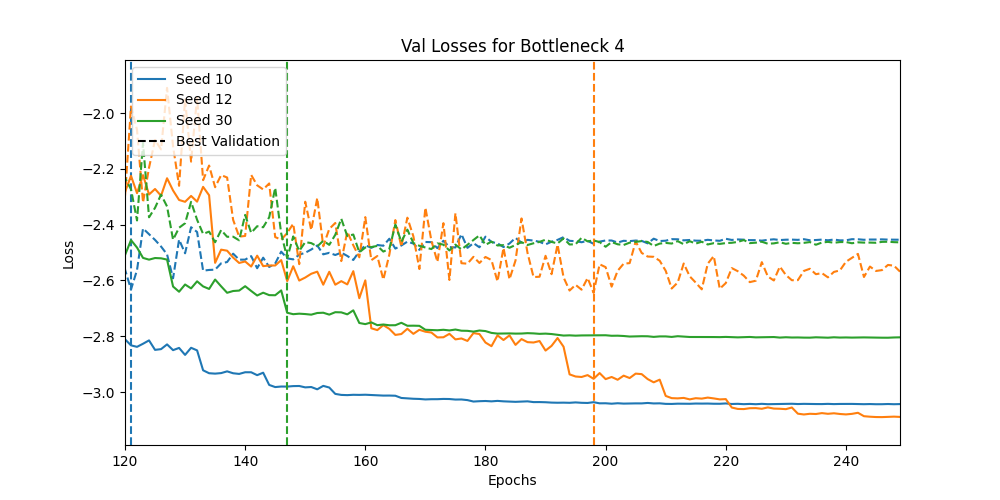
\includegraphics[width=\linewidth]{graphics/ensemble_4/joint_losses.png}
    \caption{Train and Validation Losses for Bottleneck Dimension 4}
    \label{fig:train_val_bottle_4}
\end{figure}
\begin{figure}
    \centering
    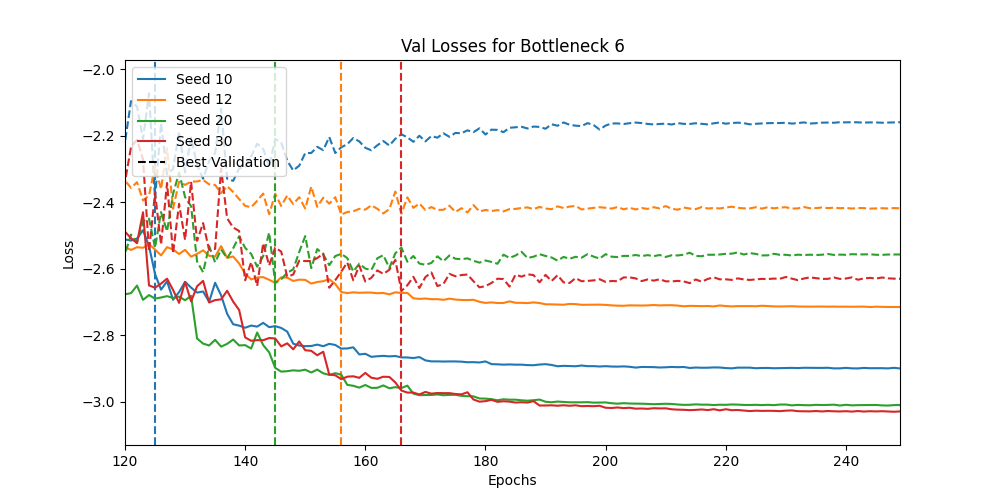
\includegraphics[width=\linewidth]{graphics/ensemble_6/joint_losses.png}
    \caption{Train and Validation Losses for Bottleneck Dimension 4}
    \label{fig:train_val_bottle_6}
\end{figure}
\begin{figure}
    \centering
    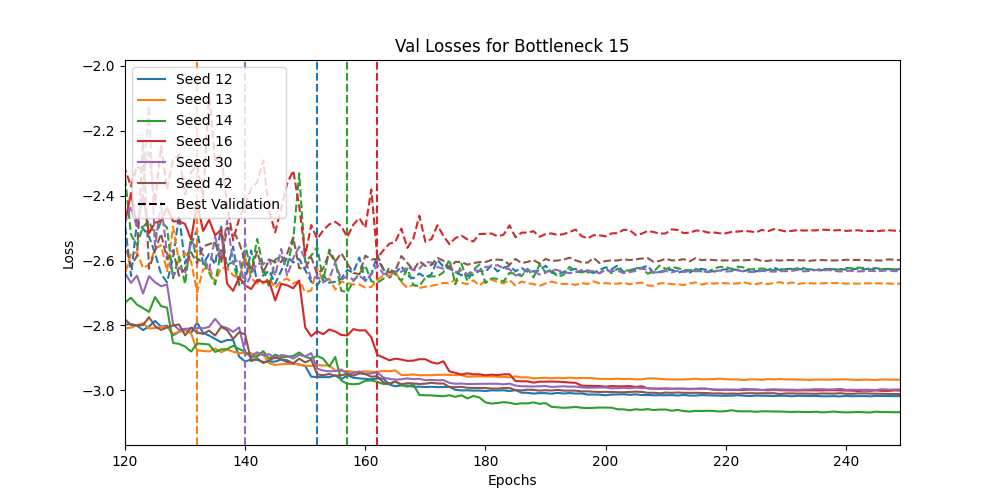
\includegraphics[width=\linewidth]{graphics/ensemble_15/joint_losses.png}
    \caption{Train and Validation Losses for Bottleneck Dimension 4}
    \label{fig:train_val_bottle_15}
\end{figure}
\begin{figure}
    \centering
    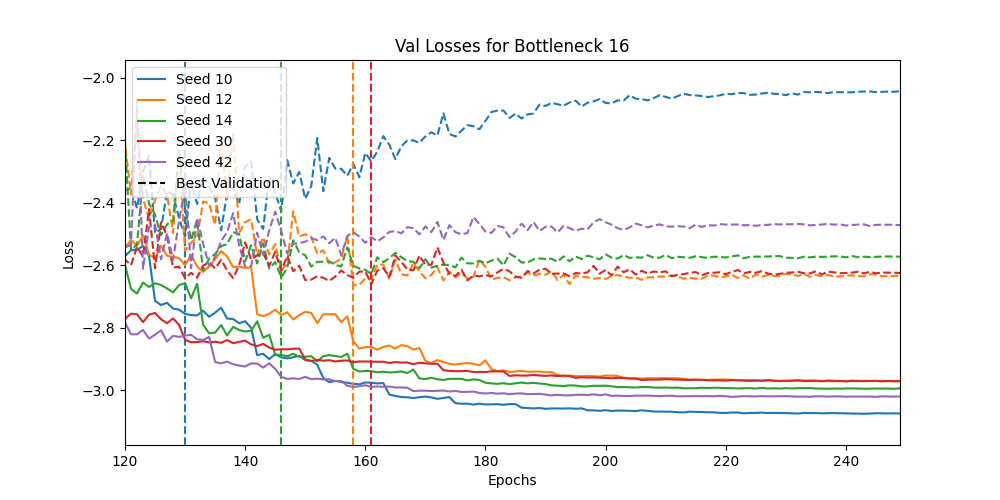
\includegraphics[width=\linewidth]{graphics/ensemble_16/joint_losses.png}
    \caption{Train and Validation Losses for Bottleneck Dimension 4}
    \label{fig:train_val_bottle_16}
\end{figure}

% \begin{figure}[]
%     \centering
%     \begin{subfigure}{0.49\textwidth}
%         \centering
%         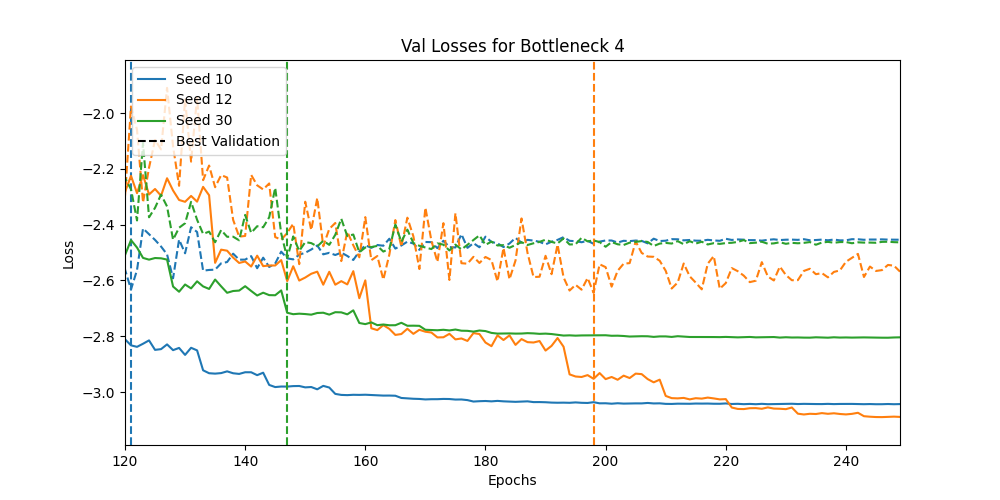
\includegraphics[width=\linewidth]{graphics/ensemble_4/joint_losses.png}
%         \caption{caption}
%         \label{fig:ensemble_4_joint_losses}
%     \end{subfigure}
%     \hfill
%     \begin{subfigure}{0.49\textwidth}
%         \centering
%         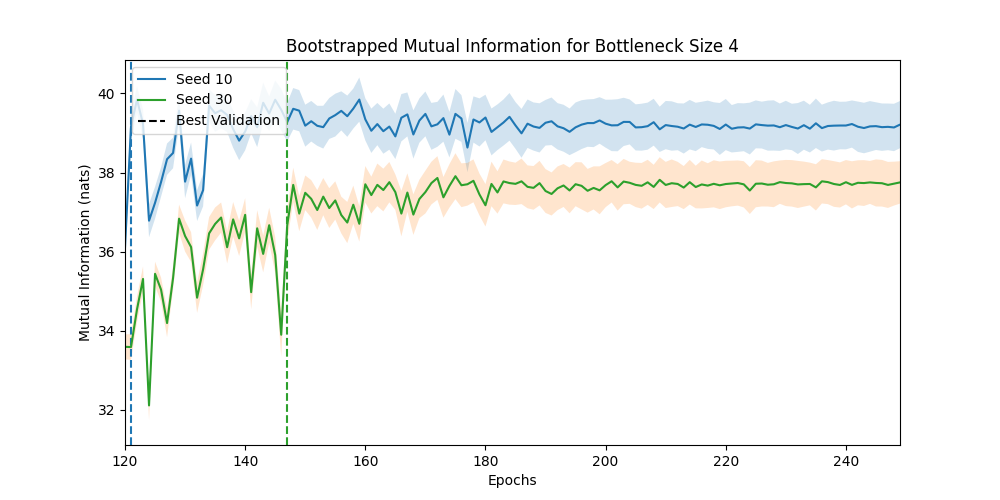
\includegraphics[width=\linewidth]{graphics/ensemble_4/mutual_information_bootstrapped.png}
%         \caption{caption}
%         \label{fig:ensemble_4_ce}
%     \end{subfigure}

%     \vspace{0.5cm}

%     \begin{subfigure}{0.49\textwidth}
%         \centering
%         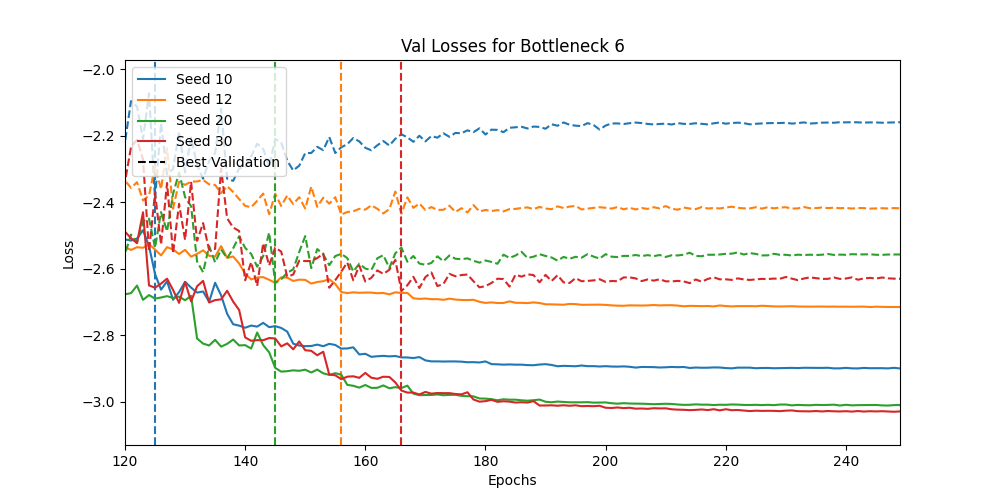
\includegraphics[width=\linewidth]{graphics/ensemble_6/joint_losses.png}
%         \caption{Bottom left}
%         \label{fig:ensemble_6_joint_losses}
%     \end{subfigure}
%     \hfill
%     \begin{subfigure}{0.49\textwidth}
%         \centering
%         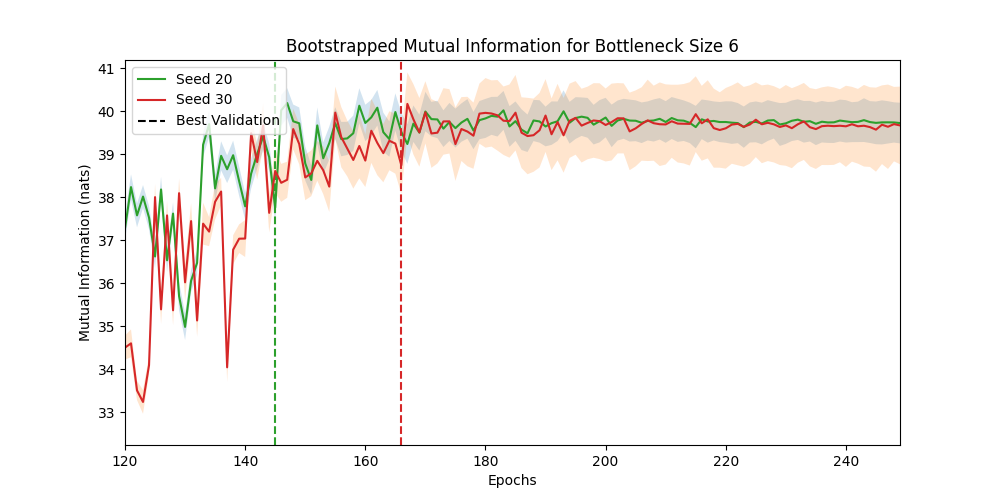
\includegraphics[width=\linewidth]{graphics/ensemble_6/mutual_information_bootstrapped.png}
%         \caption{Bottom right}
%         \label{fig:ensemble_6_ce}
%     \end{subfigure}

%     \caption{Overall caption for both figures}
% \end{figure}


Figures~\cref{fig:mi_bootstrap_bottle_4,fig:mi_bootstrap_bottle_6,fig:mi_bootstrap_bottle_15,fig:mi_bootstrap_bottle_16} show the estimated conditional entropy per epoch for each ensemble the model was trained on. Vertical lines again mark the epoch with best validation performance. All models reach a saturated estimate of the conditional entropy \red{in the epoch range...} The conditional entropy curves showcase a higher instability than the validation curves, which is attributed to the smaller size of the test set.

The model error on the conditional entropy estimate grows with increasing training steps. Some reionization histories are attributed with very low likelihood, such that the distribution of $\log q_\theta (\text{label}_i|\text{summary}_i)$ has a heavy left-sided tail. This is in parts because of the distribution of the labels themselves. 

A separate normalizing flow is trained on the label distribution. \red{Discuss other possible modelling choices and why not took them} The model with best validation performance is chosen for the following analysis. It's distribution of $\log \tilde{q}_\theta (\text{label}_i)$ also showcases a heavy left-sided tail. 

As an example, a histogram plot of the distributions $\log q_\theta (\text{label}_i|\text{summary}_i)$ and $\log \tilde{q}_\theta (\text{label}_i)$ is shown in figure~\red{insert figure}. 

According to the CLT, one would estimate the model error by the standard deviation. The heavy kurtosis inflates the value of standard deviation. As an alternative estimate of error, a bootstrapping method is implemented. \red{Quote some source that cites this as best practice.} \red{The exact values used for bootstrapping for reproducibility.} \red{Something on interpretation of bootstrap results.}

\begin{figure}
    \centering
    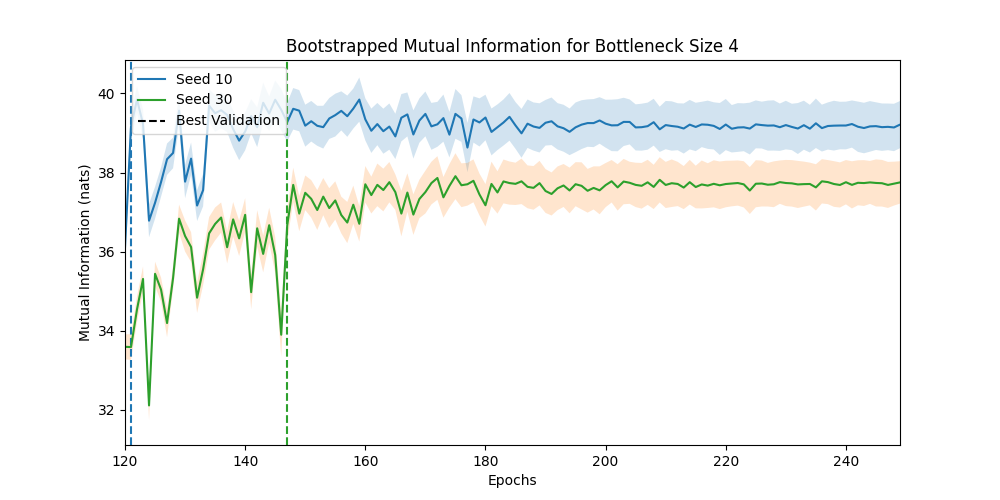
\includegraphics[width=\linewidth]{graphics/ensemble_4/mutual_information_bootstrapped.png}
    \caption{Mutual Information per Epoch for Bottleneck Dimension 4}
    \label{fig:mi_bootstrap_bottle_4}
\end{figure}
\begin{figure}
    \centering
    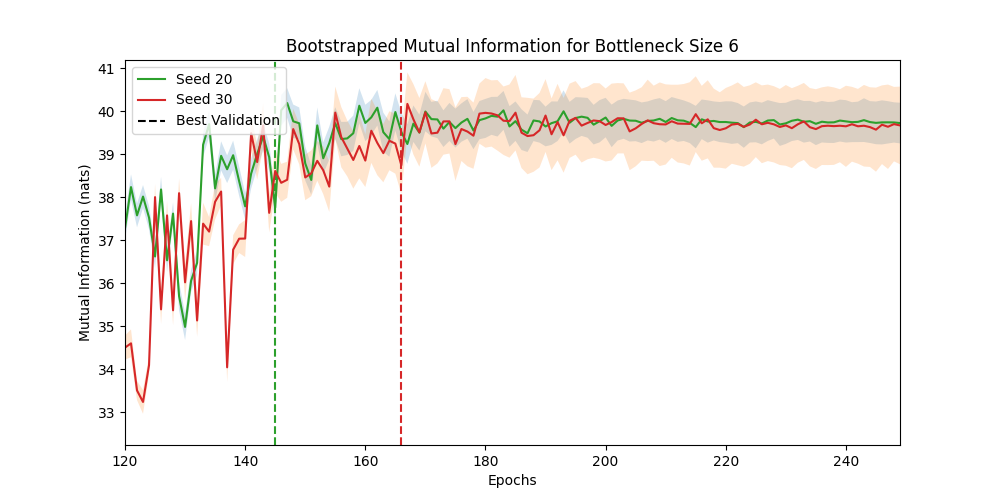
\includegraphics[width=\linewidth]{graphics/ensemble_6/mutual_information_bootstrapped.png}
    \caption{Mutual Information per Epoch for Bottleneck Dimension 4}
    \label{fig:mi_bootstrap_bottle_6}
\end{figure}
\begin{figure}
    \centering
    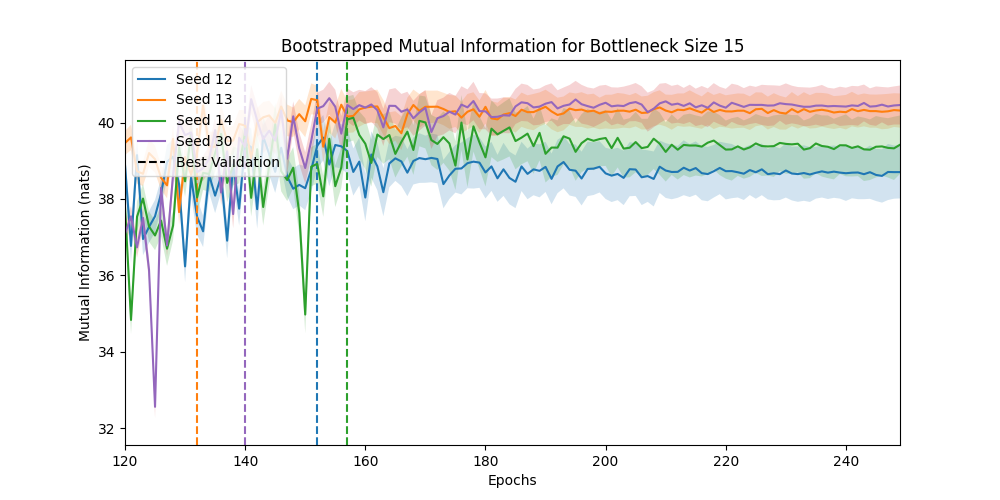
\includegraphics[width=\linewidth]{graphics/ensemble_15/mutual_information_bootstrapped.png}
    \caption{Mutual Information per Epoch for Bottleneck Dimension 4}
    \label{fig:mi_bootstrap_bottle_15}
\end{figure}
\begin{figure}
    \centering
    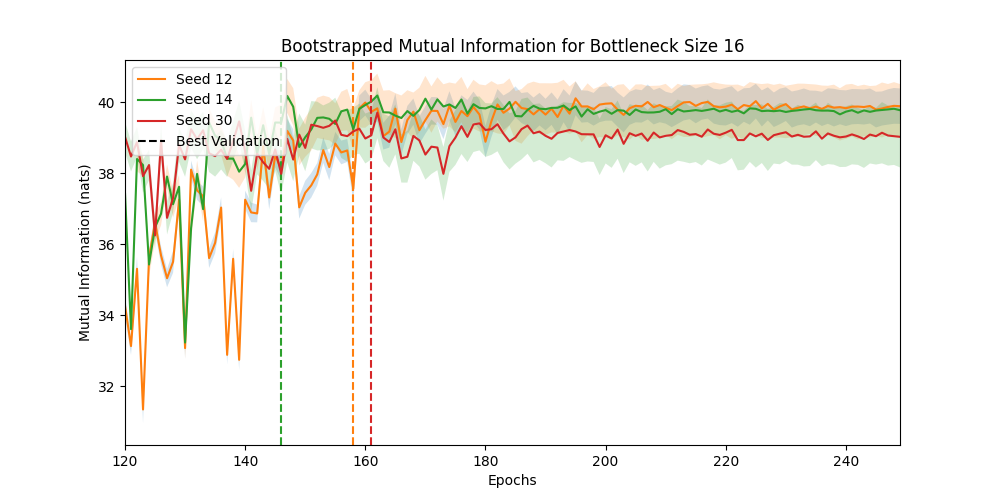
\includegraphics[width=\linewidth]{graphics/ensemble_16/mutual_information_bootstrapped.png}
    \caption{Mutual Information per Epoch for Bottleneck Dimension 4}
    \label{fig:mi_bootstrap_bottle_16}
\end{figure}

For each bottleneck dimension, the final MI estimate is made by selecting the model with best validation loss from each seed and 

averaging the conditional entropy for each of these models. The final error on the CE estimate is comprised of the model error and the \text{seed error}, stemming from the variability of results across different seeds. The final estimates with errors as shown in table~\ref{tab:CE_results}.
\begin{table}[htbp]
\centering
\caption{Final Esimation of CE per Bottleneck Dimension (all entropy values in~\si{nats})}
\label{tab:CE_results}
\begin{tabular}{l c c c c}
\toprule

Bottleneck & CE & Seed error & Model error & No. samples\\
\midrule
4 & $38.81\pm 0.71$ & $0.39$ & $0.12$ & $3$ \\
6 & $38.49\pm 0.95$ & $0.83$ & $0.06$ & $4$ \\
15 & $39.90\pm 0.42$ & $0.13$ & $0.05$ & $5$ \\
16 & $39.57\pm 0.46$ & $0.13$ & $0.09$ & $4$ \\

\bottomrule
\end{tabular}
\end{table}
These results can be described as follows: One does observe a general trend of increasing mutual information for increased bottleneck dimension, though the increase is not monotonous. In all cases, the seed error is larger than the model error, indicating training instablity to be the largest source of error in this setup. 

\red{This indicates the seed error being overestimated? Maybe have to exclude some model. Talk about decision mechanisms and how this introduces bias}

\red{Results if including selection bias}
\section{Outlook}

\green{Hi Caroline, in case you're already reading this, I finally got the CNN to train on the 6-param inference problem as well! It even works if I attach a small MLP head to the end, which means I am now running pretraining also on larger bottleneck dims (since pretraining needs MSE error with original 6 params, I needed to add a small network that changes bottleneck dim output -> six dim outut). I hope smaller bottleneck dims will work as well!  $\smiley$} 

See~\ref{fig:joint_loss_example} for an example of joint training loss after pretraining both models.

\begin{figure}
    \centering
    \includegraphics[width=\linewidth]{graphics/screnshot1.png}
    \caption{Joint loss after pretraining}
    \label{fig:joint_loss_example}
\end{figure}


How one could incorporate information geometry for similar problems

Any idea how to numerically resolve $F_{ij}$ for this flow?

Alternative choices than to model instead of $p(x|y)$ and $p(x)$?

The compressing network usually has a much heavier architecture. Once it has been trained, one can learn different lighter networks to map its summary to different target distributions. \red{This is only really true in the self-supervised case, see SKATR. So Maybe this should go in outlook}
\section{Outlook}

How one could incorporate information geometry for similar problems

Any idea how to numerically resolve $F_{ij}$ for this flow?

Alternative choices than to model instead of $p(x|y)$ and $p(x)$?

% ---------- Backmatter ----------
\newpage
\appendix
\section{Network Implementation}

Network architecture, training details, losses

\printbibliography

\end{document}